\documentclass[12pt,a4paper]{article}
\usepackage[utf8]{inputenc}
%\usepackage[spanish]{babel}
\usepackage{amsmath}
\usepackage{amsfonts}
\usepackage{amssymb}
\usepackage{graphicx}
\newcommand*{\qed}{\hfill\ensuremath{\blacksquare}}
\setlength{\parindent}{0pt}
\pretolerance=2000
\tolerance=3000
\author{Santiago de Diego, Jesús Bueno, Fernando de la Cruz, Javier Ruiz}
\title{Cadenas de Markov en tiempo continuo}
\date{}
\begin{document}
\maketitle
\newtheorem{theorem}{Teorema}[section]
\newtheorem{lemma}{Lema}[section]
\newtheorem{proof}{Demostración}[section]
\newtheorem{prop}{Proposición}[section]
\newtheorem{definition}{Definición}[section]
\newpage
\tableofcontents
\newpage
\section{Introducción}
\subsection{Cadenas de Markov}
Primero de todo, presentamos una introducción a las Cadenas de Markov de forma genérica. Como ya sabemos, las cadenas de Markov son procesos de corta memoria en el sentido de que solo recuerdan el último estado visitado para decidir cual sería el próximo. En procesos con larga memoria el valor que toma el proceso en cada paso depende de todo el pasado.

Formalizando el concepto, el proceso $\{\mathbb{X}_n \}_{n\in \mathbb{N}}$ con espacio de estados $E$ es una cadena de Markov si:

$$P(\mathbb{X}_{n+1}=y \, | \, \mathbb{X}_n = x_n , \ldots , \mathbb{X}_0 = x_0)=P(\mathbb{X}_{n+1}=y \, | \, {\mathbb{X}_n=x_n})$$

Este tipo de procesos estocásticos tienen mucho interés a la hora de modelar determinados fenómenos, como por ejemplo el tiempo de espera a un servidor en función de la tasa de llegada de los clientes.

\subsection{Diferencia entre tiempo discreto y tiempo continuo}
La principal diferencia entre cadenas de Markov en tiempo discreto y tiempo continuo es, como dice el propio nombre, el tiempo. En las cadenas de Markov en tiempo continuo, consideramos un $t\in T \subset \mathbb{R}$ mientras que en las cadenas de Markov en tiempo discreto, trabajamos con instantes de tiempo de la forma $t\in \mathbb{N}$.
\section{Definición y propiedades}
\subsection{Definición}
Primero de todo, definiremos una Cadena de Markov como:
\begin{definition}{\textbf{Cadena de Markov en tiempo continuo}}\\
Sea $\{\mathbb{X}_t\}_{t\geq 0}$ un proceso estocástico en tiempo continuo, esto es, $t\in [0,T]$ con $T\in \mathbb{R}$ que toma valores en un conjunto numerable $E$. Decimos que $\{\mathbb{X}_t\}_{t\geq 0}$ es una Cadena de Markov en tiempo continuo si $\forall t,s\geq 0$ y $\forall i,j,x_u\in E$ con $0\leq u < s$, se cumple que:
$$P(\mathbb{X}_{t+s}=j \, | \, \mathbb{X}_s =i \, , \,  \mathbb{X}_u =  u \,\, \forall 0\leq u <s)=P(\mathbb{X}_{t+s}=j \, | \, \mathbb{X}_s = i)$$
\end{definition}
Es decir, podemos definir una Cadena de Markov como un proceso estocástico	en el que el futuro sólo depende del presente, independientemente de sus estados pasados. Además también podemos considerar la definición alternativa:
\begin{definition}{\textbf{Cadena de Markov en tiempo continuo}}\\
El proceso estocástico $\{\mathbb{X}_t \, , \, t\in [0,\infty]\}$ es una Cadena de Markov en tiempo continuo si para cualquier entero $n\geq 0$, cualesquiera $0\leq t_0 < t_1 < \ldots < t_{n+1}$ y $i_0,\ldots , i_n,i_{n+1}\in S$ se verifica:
$$P(\mathbb{X}_{t_{n+1}}=i_{n+1}\, | \, \mathbb{X}_{t_0}=i_0 , \ldots \mathbb{X}_{t_n}=i_n)=P(\mathbb{X}_{t_{n+1}}=i_{n+1}\, | \, \mathbb{X}_{t_n}=i_n)$$
\end{definition}
Además, introducimos también el concepto de Cadena de Markov en tiempo continuo homogénea:
\begin{definition}{\textbf{Cadena de Markov homogénea en tiempo continuo}}\\
Una CMTC se dice homogénea si la probabilidad de ir del estado $i$ al estado $j$ no depende del instante de tiempo en el que se encuentra la cadena, formalmente esto es:
$$P(\mathbb{X}_{t_n}=j \, | \, \mathbb{X}_{t_{n-1}}=i)=P(\mathbb{X}_{t_1}=j \, | \, \mathbb{X}_{t_0}=i)$$
\end{definition}
Una vez vistas estas definiciones podemos ver las propiedades de una Cadena de Markov.
\subsection{Propiedades}
Podemos notar dos propiedades fundamentales en cuanto a CMTC, que son:
\subsubsection{Primera propiedad}
$P(\mathbb{X}_{t_{n+h}}=i_{n+h}, h=1,\ldots m \, | \, \mathbb{X}_{t_k}=i_k, k=0,\ldots ,n)=P(\mathbb{X}_{t_{n+h}}=i_{n+h}, h=1,\ldots m\, |\, \mathbb{X}_{t_n}=i_n )$
\\
$\forall 0 \leq t_1< t_2, \ldots , < t_n+m\, , \forall i_k\in S, k=0,\ldots , n+m$
\begin{proof}
Vamos a demostrarlo por inducción:
\\\\
Primero hacemos el caso $h=1$:
\\\\
$P(\mathbb{X}_{t_{n+1}}=i_{n+1},h=1 \, |\, \mathbb{X}_{t_k}=i_k\, k=0,\ldots n)=P(\mathbb{X}_{t_{n+1}}=i_{n+1}\, | \,\mathbb{X}_{t_n}=i_n)$
\\
$\forall 0\leq t_1<t_2<\ldots <t_{n+m}\, \forall m\geq 1$ y $\forall i_k \in S, \,k=0,\ldots n+m$
\\\\
Lo suponemos cierto para $h$ y lo probamos para $h+1$:
\\\\
$P(\mathbb{X}_{t_{n+h}}=i_{n+h},\, h=1,\ldots m \, | \, \mathbb{X}_{t_k}=i_k ,\, k=0,\ldots n)P(\mathbb{X}_{t_k}=i_k,\, k=0\ldots n)$
\\
$=P(\mathbb{X}_{t_k}=i_k\, k=0,\ldots ,n+m+1)=P(\mathbb{X}_{t_{n+m-1}}=i_{n+m-1}\, | \, \mathbb{X}_{t_k}=i_k,\, k=0,\ldots , n+m)=P(\mathbb{X}_{t_k}=i_k,\, k=0,\ldots n+m)=P(\mathbb{X}_{t_{n+m+1}}=i_{n+m+1}\, | \, \mathbb{X}_{t_k}=i_k,\, k=0,\ldots ,n+m)=P(\mathbb{X}_{t_{n+h}}=i_{n+h},\, h=1,\ldots m \, | \, \mathbb{X}_{t_k}=i_k ,\, k=0,\ldots n)P(\mathbb{X}_{t_k}=i_k,\, k=0\ldots n)$
\\
$=P(\mathbb{X}_{t_{n+m+1}}=i_{n+m+1}\, | \, \mathbb{X}_{t_k}=i_k,\, k=0,\ldots ,n+m)P(\mathbb{X}_{t_{n+h}}=i_{n+h},\, h=2,\ldots m \, | \, \mathbb{X}_{t_k}=i_k ,\, k=0,\ldots n)P(\mathbb{X}_{t_k}=i_k,\, k=0\ldots n)$
\\\\
Obtenemos que:
\\\\
$P(\mathbb{X}_{t_{n+h}}=i_{n+h},\, h=1,\ldots m+1 \, | \, \mathbb{X}_{t_k}=i_k ,\, k=0,\ldots n)=P(\mathbb{X}_{t_{n+m+1}}=i_{n+m+1})P(\mathbb{X}_{t_{n+h}}=i_{n+h},\, h=1,\ldots m\, | \, \mathbb{X}_{t_n}=i_n)$
\\\\
Sin más que aplicar la definición tenemos que lo anterior es igual a $P(\mathbb{X}_{t_{n+m+1}}\, | \, \mathbb{X}_{t_n}=i_{t_n})$
\qed
\end{proof}
\subsubsection{Segunda propiedad}
Sea $\mathbb{X}_{t}$ con $t\in[o,+\infty)$ una cadena de Markov en tiempo continuo, se tiene: \newline
		\begin{equation*}
			P(\mathbb{X}_{t_{n+h}} = i_{t_{n+h}} \, |\, \mathbb{X}_{t_{k}} = i_{k} \hspace{0.2cm} k = 0,...,n) = P(\mathbb{X}_{t_{n+h}} = i_{t_{n+h}} \, |\, \mathbb{X}_{t_{n}} = i_{n}) \hspace{0.5cm} \forall h \geq 1
		\end{equation*}
\begin{proof}
		Lo haremos por inducción sobre el número de instantes de tiempo, tal y como en la primera propiedad.
		\\[0.2cm]
		Demostrémoslo para $h = 1$
		\\[0.2cm]
		$P(\mathbb{X}_{t_{n+1}} = i_{t_{n+1}} \, |\, \mathbb{X}_{t_{k}} = i_{k} \hspace{0.2cm} k = 0,...,n)\overbrace{=}^{*}P(\mathbb{X}_{t_{n+h}} = i_{t_{n+h}} \, |\, \mathbb{X}_{t_{n}} = i_{n})$
		\\[0.2cm]
		Supongámoslo demostrado para $h - 1$ y demostrémoslo para $h$.
		\\[0.2cm]
		$P(\mathbb{X}_{t_{n+h}} = i_{t_{n+h}} \, |\, \mathbb{X}_{t_{k}} = i_{k} \hspace{0.2cm} k = 0,...,n) = P(\mathbb{X}_{t_{n+h}} = i_{t_{n+h}} , \displaystyle\bigcup_{i_{n+h-1} \in S} \mathbb{X}_{t_{n+h-1}} = i_{n+h-1} ,\ldots, \bigcup_{i_{n+1} \in S} \mathbb{X}_{t_{n+1}} = i_{n+1} \, |\, \mathbb{X}_{t_{k}} = i_{k} \hspace{0.2cm} k = 0,...,n) = \sum_{i_{n+h-1} \in S} \sum_{i_{n+1} \in S} P(\mathbb{X}_{t_{n+h}} = i_{t_{n+h}} , \mathbb{X}_{t_{n+h-1}} = i_{n+h-1} ,..., \mathbb{X}_{t_{n+1}} = i_{n+1} \, |\, \mathbb{X}_{t_{k}} = i_{k} \hspace{0.2cm} k = 0,...,n) \overbrace{=}^{*}\sum_{i_{n+h-1} \in S} \sum_{i_{n+1} \in S} P(\mathbb{X}_{t_{n+h}} = i_{t_{n+h}} , \mathbb{X}_{t_{n+h-1}} = i_{n+h-1} ,\ldots, \mathbb{X}_{t_{n+1}} = i_{n+1} \, |\, \mathbb{X}_{t_{n}} = i_{n}) = P(\mathbb{X}_{t_{n+h}} = i_{t_{n+h}} , \bigcup_{i_{n+h-1} \in S} \mathbb{X}_{t_{n+h-1}} = i_{n+h-1} ,..., \bigcup_{i_{n+1} \in S} \mathbb{X}_{t_{n+1}} = i_{n+1} \, |\, \mathbb{X}_{t_{n}} = i_{n}) = P(\mathbb{X}_{t_{n+h}} = i_{t_{n+h}} \, |\, \mathbb{X}_{t_{n}} = i_{n})$
		\\[0.2cm]
		Nota: "$*$" significa "por definición de cadena de Markov".
		\qed
\end{proof}
\subsection{Relación con la teoría de autómatas}
En concreto, podemos asociar a una cadena de Markov un grafo, como veremos más abajo. De esta forma, el grafo resultante se comporta de igual manera que un \textbf{autómata finito determinista}, relacionándose de esta forma las cadenas de Markov con la teoría de autómatas.
\\\\
Primero de todo, vamos a definir el grafo de una CMTC ya que resulta fundamental para entender lo siguiente:
\\\\
\textbf{Definición: Grafo asociado a una CMTC}
\\
$G=(E,U,W)$ es el grafo asociado a una CMTC sii:
\begin{itemize}
\item $E$ es el conjunto de estados de la cadena
\item $U$ es el conjunto de aristas, que en este caso sería el conjunto de transiciones posibles
\item $W$ es el conjunto de ponderaciones. Podemos verlo como el conjunto de valores de cada arista
\end{itemize}
Además $G$ es un grafo orientado, es decir, que tenemos en cuenta cual es el nodo origen y cual es el nodo destino.
\\\\
Una vez presentada la definición de grafo asociado a una CMTC, podemos establecer una biyección entre el conjunto de grafos orientados asociados a una CMTC y el conjunto de los autómatas finitos deterministas, aunque estos resultados se escapan del alcance del trabajo en cuestión. Simplemente mostraremos un ejemplo de uno de estos grafos:
\\
\begin{figure}[h]
  \centering
    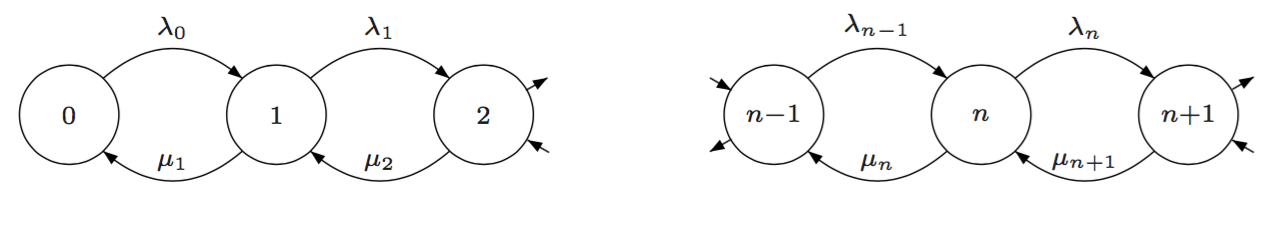
\includegraphics[width=0.7\textwidth]{img/grafo.png}
  \caption{Ejemplo de grafo de una CMTC}
  \label{fig:ejemplo}
\end{figure}
\\
En el grafo de la izquierda aparecen 3 estados, que corresponden a las variables aleatorias $\mathbb{X}_{t_1}$, $\mathbb{X}_{t_2}$ y $\mathbb{X}_{t_3}$ y representadas como $\lambda_0$, $\lambda_1$, $\mu_1$, $\mu_2$ aparecen las 4 probabilidades de transición. Por último, las flechas indican la dirección en la que se produce la transición.
\\\\
El grafo de la derecha es idéntico pero corresponde a las variables aleatorias $\mathbb{X}_{t_{n-1}}$, $\mathbb{X}_{t_n}$ y $\mathbb{X}_{t_{n+1}}$. Además, según lo visto anteriormente tenemos que el grafo corresponde a la manera usual de representar un autómata finito determinista.
\\\\
Para concluir presentaremos la definición de autómata finito determinista, por si el lector está interesado en el estudio del mismo:
\\\\
\textbf{Definición de autómata finito determinista:}
\\
Un AFD es una 5-tupla $(Q,\sum ,q_0,\delta,F)$ donde:
\begin{itemize}
\item $Q$ es un conjunto de estados
\item $\sum$ es un alfabeto
\item $q_0$ es el estado inicial
\item $\delta :Q\times\sum\rightarrow Q$ es la función de transición
\item $F\subseteq Q$ es el conjunto de estados finales
\end{itemize}
Además verifica que $\delta (q,a)=q_1$ y $\delta (q,a)=q_2 \Rightarrow q_1 \neq q_2$ y que no existen transiciones de la forma $\delta(q,\epsilon)$ donde $\epsilon$ es la cadena vacía.
\\\\
Veamos un ejemplo de un autómata finito determinista muy simple:
\begin{figure}[h]
  \centering
    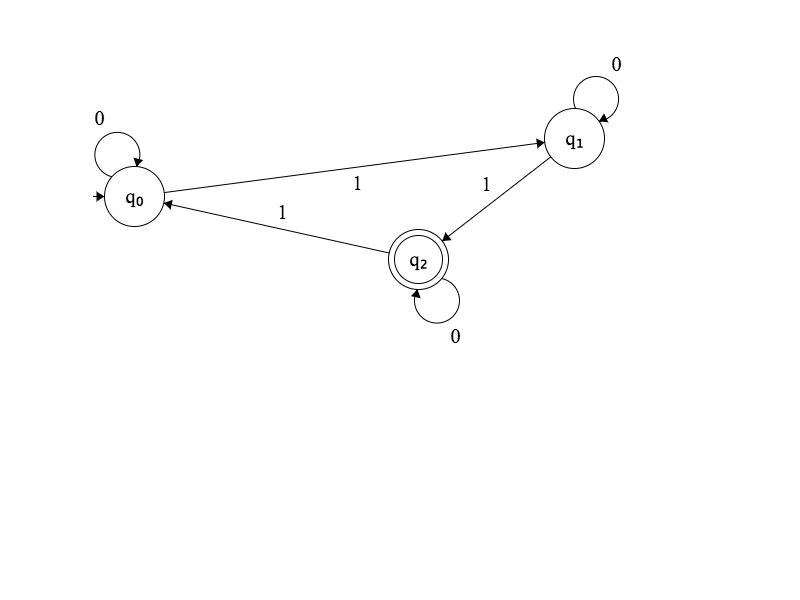
\includegraphics[width=0.8\textwidth]{img/afd.png}
  \label{fig:ejemplo}
\end{figure}

Observando la definición y aplicándola a este caso concreto podemos diferenciar:
\begin{itemize}
\item $Q=\{q_0,q_1,q_2 \}$
\item $\sum = \{0,1\}$
\item $q_0=q_0$
\item Función de transición $\delta \, t.q$:
\\
$\delta(q_0,0)=q_0 \,\,\,\,\,\,\, \delta(q_1,0)=q_1\,\,\,\,\,\,\, \delta(q_2,0)=q_2$
\\
$\delta(q_0,1)=q_1 \,\,\,\,\,\,\,  \delta(q_1,1)=q_2 \,\,\,\,\,\,\,\delta(q_2,1)=q_0$
\item $F={q_2}$
\end{itemize}
De esta forma, queda clara la correspondencia entre AFD y CMTC, sin más que comparar la definición de grafo de una CMTC con la definición de AFD.
\\\\
Podemos ver las correspondencias: $Q=E\, ,\, \sum=W$ y $| \delta |=U$ y ademas el conjunto de estados finales es el vacío, es decir, $F={\emptyset}$. 

\section{Probabilidades de transición}

Comenzamos definiendo las llamadas probabilidades de transición. Posteriormente, a partir de estas probabilidades, y restringiéndonos únicamente al caso en que la CMTC sea homogénea, construiremos la matriz de transición $P(t)$ y demostraremos sus propiedades más importantes.

Por último, partiendo de $P(t)$, generaremos y estudiaremos una nueva matriz, denominada $Q$-matriz o generador infinitesimal.

\subsection{Probabilidades de transición y matriz de transición}
\textbf{Definición: Probabilidades de transición}
\\
Dada una CMTC $\{\mathbb{X}_t \, , \, t\in [0,\infty]\}$, definimos las probabilidades de transición como:
$$p_{ij}(s,t):=P(\mathbb{X}_t=j\, | \, \mathbb{X}_s=i), \ 0\leq s < t, \ \ i,j\in S$$

A partir de este momento, supondremos que la CMTC es homogénea. Teniendo en cuenta la expresión anterior y siguiendo la definición de Cadena de Markov homogénea en tiempo continuo, citada en la sección (2.1), tenemos que la probabilidad de ir del estado $i$ al estado $j$ no depende del instante de tiempo en el que se encuentra la cadena, es decir, $p_{ij}(s,t)$ no depende de $s$ y $t$, sólo depende de la diferencia $t-s$:
$$p_{ij}(s,t)=P(\mathbb{X}_t=j\, | \, \mathbb{X}_s=i)=P(\mathbb{X}_{t-s}=j\, | \, \mathbb{X}_0=i)=p_{ij}(0,t-s)=p_{ij}(t-s)$$
Por tanto, podemos expresar las probabilidades de transición como:
$$p_{ij}(t)=P(\mathbb{X}_t=j\, | \, \mathbb{X}_0=i)=P(\mathbb{X}_{t+s}=j\, | \, \mathbb{X}_s=i)$$
siendo $t$ la diferencia entre los dos instantes de tiempo. En particular:
$$p_{ij}(0)=P(\mathbb{X}_0=j\, | \, \mathbb{X}_0=i)=\delta_{ij}:= \left\{ \begin{array}{lcc}
   	   	             1 &   si  & i=j \\
   	   	             0 &  si & i\neq j
   	   	             \end{array} \right. $$
Estamos en condiciones de construir la matriz de transición, cuyos elementos son todas las posibles probabilidades de transición:
$$P(t):=(p_{ij}(t))_{i,j\in S}$$
\textbf{Propiedades:}
\begin{enumerate}
\item Para cada $t\geq 0, \ \ p_{ij}(t)\geq 0, \ \ \forall i,j\in S$,
\item Para cada $t\geq 0, \ \ \sum\limits_{j\in S}p_{ij}(t)=1, \ \ \forall i\in S$,
\item Ecuación de \textit{Chapman-Kolmogorov}: 
$p_{ij}(s+t)=\sum\limits_{k\in S}p_{ik}(s)p_{kj}(t), \ \ \forall i,j\in S, \ \ \forall s,t\in[0,\infty)$.
\end{enumerate}

\begin{proof}
\begin{enumerate}
\item Evidente, pues $P$ es probabilidad.
\item Partiendo del hecho de que $P[\Omega]=P\left[\{\omega\in\Omega/\mathbb{X}_t(\omega)\in S\}\right]=P\left[\bigcup\limits_{j\in S}\{\omega\in\Omega/\mathbb{X}_t(\omega)=j\}\right]=P\left[\bigcup\limits_{j\in S}[\mathbb{X}_t=j]\right]=1$, tenemos:
\\\\\\
$1=P\left[\bigcup\limits_{j\in S}[\mathbb{X}_t=j]\, | \,\mathbb{X}_0=i\right]\overset{*}{=}\sum\limits_{j\in S}P\left[\mathbb{X}_t=j\, | \,\mathbb{X}_0=i\right]-\underbrace{P\left[\bigcap\limits_{j\in S}[\mathbb{X}_t=j]\, | \,\mathbb{X}_0=i \right]}_{0}=\sum\limits_{j\in S}P\left[\mathbb{X}_t=j\, | \,\mathbb{X}_0=i\right]=\sum\limits_{j\in S}p_{ij}(t)$.
\\\\

(*) $P(A_1\cup A_2\cup ... \cup A_n\, |\, B)=P(A_1\, |\,B)+P(A_2\, |\,B)+...+P(A_n\, |\,B)-P(A_1\cap A_2\cap ... \cap A_n\, |\, B)$.
\item $p_{ij}(s+t)=P\left[\mathbb{X}_{s+t}=j\, | \,\mathbb{X}_0=i\right]=P\left[\mathbb{X}_{s+t}=j, \bigcup\limits_{k\in S}[\mathbb{X}_s=k]\, | \,\mathbb{X}_0=i\right]=$

$=\sum\limits_{k\in S}P\left[\mathbb{X}_{s+t}=j,\,\mathbb{X}_s=k\, | \,\mathbb{X}_0=i\right]\overset{**}{=}$

$=\dfrac{P[\mathbb{X}_{s+t}=j,\,\mathbb{X}_s=k,\,\mathbb{X}_0=i]}{P[\mathbb{X}_0=i]}\overset{**}{=}$

$=\sum\limits_{k\in S}P\left[\mathbb{X}_{s+t}=j\, | \,\mathbb{X}_s=k, \mathbb{X}_0=i\right]P\left[\mathbb{X}_s=k\, | \,\mathbb{X}_0=i\right]\overset{CMTC}{=}$

$=\sum\limits_{k\in S}P\left[\mathbb{X}_{s+t}=j\, | \,\mathbb{X}_s=k\right]P\left[\mathbb{X}_s=k\, | \,\mathbb{X}_0=i\right]\overset{\text{Homogénea}}{=}$

$=\sum\limits_{k\in S}P\left[\mathbb{X}_t=j\, | \,\mathbb{X}_0=k\right]P\left[\mathbb{X}_s=k\, | \,\mathbb{X}_0=i\right]=\sum\limits_{k\in S}p_{kj}(t)p_{ik}(s)$.
\\\\

(**) $P(A\cap B\, | \, C)=\dfrac{P(A\cap B\cap C)}{P(C)}=P(A\, | \, B\cap C)P(B\, | \,C)$ \\
\end{enumerate}
\qed
\end{proof}

\subsection{Q-matriz o generador infinitesimal}


\textbf{Definición: Q-matriz o generador infinitesimal}
\\
Dada una CMTC $\{\mathbb{X}_t \, , \, t\in [0,\infty]\}$, con matriz de transición $P(t)$. Se define la $Q$-matriz o generador infinitesimal como:
$$Q:=\lim_{t \to 0}\dfrac{P(t)-I}{t},$$
donde $I$ es la matriz identidad del tamaño correspondiente y, por tanto, los elementos de la diagonal principal se expresan como:
$$q_{ii}=\lim_{t \to 0}\dfrac{p_{ii}(t)-1}{t}:=-q_i,$$
donde $q_i$ es la \textit{razón de escape} del estado $i$, mientras que el resto de elementos:
$$q_{ij}=\lim_{t \to 0}\dfrac{p_{ij}(t)}{t},\,\,\, i\neq j$$
donde $q_{ij}$ es llamado \textit{razón de transición} del estado $i$ al $j$.
\\\\
En lo que resta de sección, procederemos a construir esta matriz a partir de la definición de una nueva variable aleatoria. A partir de este momento, asumimos que la CMTC $\{\mathbb{X}_t \, , \, t\in [0,\infty]\}$ es continua por la derecha, es decir, si la transición de un estado $i\in S$ a un estado $j\in S$ ocurre el instante $t$, entonces se tiene que $\mathbb{X}_t=j$ y $\mathbb{X}_{t^-}=i$.

La cuestión es: ¿Dado $\mathbb{X}_0=i$, cuánto tiempo permanecerá el proceso en el estado $i$? Para responder a esta pregunta, definimos la siguiente variable aleatoria:
$$\xi_i\equiv \text{Tiempo que el proceso permanece en el estado} \,\, i.$$

Vamos a deducir la distribución que sigue $\xi_i$. Para ello será suficiente con probar que la variable $\xi_i$ verifica la propiedad de falta de memoria, en efecto, dados $t,s\geq 0$:
\\
$$P[\xi_i>s+t\, | \,\xi_i>s]=$$ 
$$=P[\mathbb{X}_r=i,\, para \, r\in[0,s+t]\, | \,\mathbb{X}_r=i,\, para \, r\in[0,s]]=$$
$$=P[\mathbb{X}_r=i,\, para \, r\in[s,s+t]\, | \,\mathbb{X}_r=i,\, para \, r\in[0,s]]\overset{CMTC}{=}$$
$$=P[\mathbb{X}_r=i,\, para \, r\in[s,s+t]\, | \,\mathbb{X}_s=i]\overset{\textit{Homogénea}}{=}$$
$$=P[\mathbb{X}_r=i,\, para \, r\in[0,t]\, | \,\mathbb{X}_0=i]=$$
$$=P[\xi_i>t].$$

Puesto que $\xi_i$ es una variable continua verificando la propiedad de falta de memoria, tenemos que $\xi_i\rightsquigarrow exp(\lambda_i)$, con $\lambda_i>0$, puesto que las únicas variables continuas que verifican esta propiedad son aquellas que siguen una distribución exponencial. Conocida la distribución de $\xi_i$, deducimos:
$$\mathbb{E}[\xi_i]=\dfrac{1}{\lambda_i},$$
y, por tanto, cuánto más grande sea el parámetro $\lambda_i$, más pequeño será el intervalo de tiempo en el que el proceso se encuentra en el estado $i$.
\\\\
Estamos preparados para construir la $Q$-matriz, $Q=(q_{ij})_{i,j\in S}$. Sea:
$$p_{ij}(\xi_i)=P(\mathbb{X}_{\xi_i}=j\, | \, \mathbb{X}_0=i), \,\, j\neq i$$
la probabilidad de transición del estado $i$ al estado $j$, definimos:
$$q_{ij}:=\lambda_i p_{ij}(\xi_i),\,\, i\neq j$$
la \textit{razón de transición} del estado $i$ al $j$. Para obtener los elementos de la diagonal, es decir, para el caso en que $i=j$, imponemos que la suma de los elementos de cada una de las filas de $Q$ sea $0$:
$$q_{ii}+\sum_{j\neq i}q_{ij}=0$$
$$q_{ii}=-\sum_{j\neq i}q_{ij}$$
$$q_{ii}=-\sum_{j\neq i}\lambda_i p_{ij}(\xi_i)$$
$$q_{ii}=-\lambda_i\underbrace{\sum_{j\neq i}p_{ij}(\xi_i)}_{1}$$
$$q_{ii}=-\lambda_i:=-q_i$$
y hemos obtenido $q_i$, la \textit{razón de escape} del estado $i$. Por tanto, la $Q$-matriz se puede expresar de la siguiente manera:

$$Q= \left\{ \begin{array}{lcc}
   	   	             -\sum\limits_{j\neq i}q_{ij} &   si  & i=j \\
   	   	             q_{ij} &  si & i\neq j
   	   	             \end{array} \right. $$
o equivalentemente:
$$Q= \left\{ \begin{array}{lcc}
   	   	             -\lambda_i &   si  & i=j \\
   	   	             \lambda_i p_{ij}(\xi_i) &  si & i\neq j
   	   	             \end{array} \right. $$

\section{Ecuación de Kolmogorov}
	Ya que una cadena de Markov está determinada por las probabilidades de transición, que ya hemos definido, vamos a calcularlas a partir de la razón de transición. Vamos a formalizarlo con el siguiente teorema.
	\begin{theorem}[Teorema de las Ecuaciones Diferenciales de Kolmogorov] Sea $\mathbb{X}_{t}$ con $t \in [0,\infty)$ es una cadena de Markov que no tiene nigún estado instantáneo. Entonces las probabilidades de transición son diferenciables en $t$ y $\forall i,j$, par de estados, se tiene:
		\begin{equation*}
			P'(t) = P(t)Q\hspace{0.1cm}y\hspace{0.1cm}P(0) = I \iff \frac{dp_{ij}(t)}{dt} = -p_{ij}q_{j} + \sum_{k \neq j} p_{ik}(t)q_{kj} \hspace{0.5cm} p_{ij}(0) = \delta_{ij} \hspace{0.5cm}
		\end{equation*}
		(Ecuación adelantada)
		\begin{equation*}
			P'(t) = QP(t)\hspace{0.1cm}y\hspace{0.1cm}P(0) = I \iff \frac{dp_{ij}(t)}{dt} = -q_{i}p_{ij} + \sum_{k \neq j} q_{ik}p_{kj}(t) \hspace{0.5cm} p_{ij}(0) = \delta_{ij} \hspace{0.5cm}
		\end{equation*}
		(Ecuación atrasada)
	\end{theorem}
	\begin{proof}
		En esta demostración vamos a partir de la definición de derivada de $p_{ij}(t)$ hasta llegar al resultado final aplicando la Ecuación de Chapman-Kolmogorov y las razones de transición del apartado anterior.
		\\[0.2cm]
		Conocemos la ecuación de Chapman-Kolmogorov:
		\begin{equation*}
			p_{ij}(t+h) = \sum_{k \in S}p_{ik}(h)p_{kj}(t) = 
			\begin{cases}
				\sum_{k \neq j}p_{ik}(t)p_{kj}(h) + p_{jj}(h)p_{ij}(t) \hspace{0.5cm} (1)
				\\
				\sum_{k \neq i}p_{ik}(h)p_{kj}(t) + p_{ii}(h)p_{ij}(t) \hspace{0.5cm} (2)
			\end{cases}
		\end{equation*}
		Lo que hemos hecho, básicamente, es expresar la ecuación de Chapman-Kolmogorov de dos formas distintas que nos servirán para llegar a las ecuaciones adelantadas y atrasadas.
		\\[0.2cm]
		Veamos ahora que las ecuaciones de Kolmogorov se cumplen:
		\begin{equation*}
			p'_{ij}(t) = \lim_{h \rightarrow 0} \frac{p_{ij}(t+h) - p_{ij}(t)}{h} = \lim_{h \rightarrow 0} \frac{\sum_{k \in S}p_{ik}(h)p_{kj}(t) - p_{ij}(t)}{h}
		\end{equation*}
		Si ahora aplicamos (1):
		\begin{equation*}
			\lim_{h \rightarrow 0} \sum_{k \neq j}\frac{p_{ik}(t)p_{kj}(h)}{h} - \lim_{h \rightarrow 0}\frac{p_{jj}(h) - 1}{h}p_{ij}(t) \overbrace{=}^{*} -p_{ij}q_{j} + \sum_{k \neq j} p_{ik}(t)q_{kj}\hspace{0.5cm} \text{(Ecuación adelantada)}
		\end{equation*}
		Si en cambio aplicamos (2):
		\begin{equation*}
			\lim_{h \rightarrow 0} \sum_{k \neq i}\frac{p_{ik}(h)p_{kj}(t)}{h} - \lim_{h \rightarrow 0}\frac{p_{ii}(h) - 1}{h}p_{ij}(t) \overbrace{=}^{*} -q_{i}p_{ij} + \sum_{k \neq j} q_{ik}p_{kj}(t)\hspace{0.5cm} \text{(Ecuación atrasada)}
		\end{equation*}
		O en notación matricial:
		\begin{equation*}
			\begin{cases}
				P'(t) = P(t)Q\hspace{0.1cm}:\hspace{0.1cm}P(0) = I\hspace{0.5cm} \text{(Ecuación adelantada)} \\
				P'(t) = QP(t)\hspace{0.1cm}:\hspace{0.1cm}P(0) = I\hspace{0.5cm} \text{(Ecuación atrasada)}
			\end{cases}
		\end{equation*}
		Nota: "$*$" significa que hemos aplicados las razones de transición dadas en el apartado anterior.
	\end{proof}
	Formalmente vemos que la solución a las ecuaciones de Kolmogorov viene dada por:
	\begin{equation*}
		P(t) = e^{t Q} = \sum_{i = 0}^{\infty}\frac{t^{i} Q^{i}}{i!}
	\end{equation*} 
	Cuando Q es de dimensión finita, la serie anterior es convergente y es la única solución para los dos sistemas de ecuaciones. Si Q es de dimensión infinita, no podemos afirmar nada.
	\\[0.2cm]
	Supongamos que Q es de dimensión finita y diagonalizable con valores propios $\beta_0 ,..., \beta_n$. Entonces $\exists A$ matriz invertible que verifica $Q = ADA^{-1}$ donde $D$ es la matriz diagonal formada por sus valores propios ordenados. Y como consecuencia:
	\begin{equation*}
		Q = A \begin{pmatrix}
			\beta_0 \hspace{2cm} 0 \\
			......................\\
			......................\\
			......................\\
			0 \hspace{2cm} \beta_n
		\end{pmatrix} A^{-1}
	\Rightarrow
		P(t) = A \begin{pmatrix}
			e^{\beta_0 t} \hspace{2cm} 0 \\
			......................\\
			......................\\
			......................\\
			0 \hspace{2cm} e^{\beta_n t}
		\end{pmatrix} A^{-1}
	\end{equation*}
	Ahora vamos a reformular la matriz P, definida en el apartado de la ecuación de Kolmogorov, en función de Q de forma que nos sea útil a la hora de demostrar un resultado futuro. Las expresiones son análogas, solo cambiamos la notación.
   \begin{theorem}
   	
   		Sea $p_{ij}(t)$	una matriz de transición y $\alpha$ = $\sup\limits_{j\in S} \hspace{0.2cm} q_j <0$:
   		\begin{equation*}
   		p_{ij}=e^{-\beta t}\ \sum_{n = 0}^{\infty}\frac{\beta^{n} t^{n}}{n!}p_{ij}^{(n)}, t \geq 0, i,j \in S
   		\end{equation*}
   		
   		Donde $P$=$(p_{ij})$ es una matriz estocástica definida como:
   		\begin{equation*}
   		P=I+\frac{1}{\beta}Q, \hspace{0.2cm} I= P^{(0)}, \hspace{0.2cm} \beta \geq \alpha
   		\end{equation*}
   		
   \end{theorem}
         
\section{Probabilidades absolutas y distribución estacionaria}
	Sea $\mathbb{X}_{t}$ con $t\in[0,+\infty)$ una cadena de Markov en tiempo continuo.
	\\
	Definiremos las probabilidades absolutas de una cadena de Markov (en el caso unidimensional) como la probabilidad de que una cadena se encuntre en el estado j en un tiempo t, es decir:

\begin{equation*}	
	 a_{j}=P[\mathbb{X}_{t}=j] \hspace{0.5cm}  con \hspace{0.2cm} j\in{S}, \hspace{0.2cm}  t\in[0,+\infty)
 \end{equation*}
	La distribución absoluta de $\mathbb{X}_{t}$ se define de la siguiente forma:
			\begin{equation*}
			a(t)=(a_{j}; j\in{S})
		\end{equation*}
		
		Una distribución inicial $a_{j}(0)$ se dice estacionaria si: 
				\begin{equation*}
			a_{j}(0)=a_{j}(t) \hspace{0.2cm}  \forall t\geq 0 \hspace{0.2cm} j\in S
		\end{equation*}
	\\
			Una cadena de Markov con probabilidades de transición estacionarias se denomina estacionaria si las distribuciones absolutas
		$a(t)$ son independientes de t. En dicho caso, la distribución estacionaria $a$=$(a_{j}$; $j\in{S})$, verifica que:
		\begin{equation*}
		a_{j}=a_{1}(0)p_{1j}(t)+a_{2}(0)p_{2j}(t)+\cdots=\sum_{i\in{S}} a_{i}(0)p_{ij}(t), \hspace{0.2cm} j\in S
	\end{equation*}
\section{Clasificación de los estados}
	Sea $\mathbb{X}_{t}$ con $t\in[0,+\infty)$,  cadena de Markov en tiempo continuo con probabilidades de transición estacionarias y sea $E_{i}$ un estado del espacio de estados.
	\\
		A continuación clasificaremos los estados de una cadena de Markov según:
	
	\begin{enumerate}
		\item $\xi_{i}$: tiempo que tarda un proceso en abandonar el estado $E_{i}$ o el tiempo de permanencia en dicho estado.
		\item $\alpha_{ij}$: tiempo de primera llegada al estado $E_{j}$ partiendo de $E_{i}$
		\item Según la posibilidad de ir de un estado a otro
	\end{enumerate}
		

\subsection{Clasificación según \textbf{$\xi_{i}$}}
 Como hemos notado anteriormente, $\xi_{i}$ es el tiempo de permanencia en un estado $E_{i}$, concretamente, suponemos que el proceso en el instante s está en el estado $E_{i}$, definiremos entonces:

\begin{equation*}
	\xi_{i}=inf \{ t:t > 0, x_{s+t}\neq i \}
\end{equation*}

También hemos visto que el tiempo de estancia en un estado $E_{i}$ sigue una distribución exponiencial de parámetro $q_{i}$. El tiempo medio esperado se calcula entonces como: 

\begin{equation*}
E[\xi_{i}]= \frac{1}{q_{i}}
\end{equation*}
Información que usaremos para la clasificación de los estados.
\\


\begin{itemize}
	\item Diremos que el estado $E_{i}$ es estable si:
	 \begin{equation*}
	 	0< q_{i} < +\infty, \hspace{0.2cm} (0<E[\xi_{i}]<+\infty) 
	 \end{equation*}
    \item El estado $E_{i}$ será absorbente si:
        \begin{equation*}
    	q_{i}=0, \hspace{0.2cm} (E[\xi_{i}]=+\infty)
        \end{equation*} 
     \item Por último, el estado  $E_{i}$ será instantáneo si:  
      \begin{equation*}
      	q_{i}=+\infty, \hspace{0.2cm} (E[\xi_{i}]=0)
      \end{equation*}
      
\end{itemize}


		
\subsection{Clasificación según \textbf{$\alpha_{ij}$}}
 Denotaremos $\alpha_{ij}$ tiempo de primera llegada al estado $E_{j}$ partiendo de $E_{i}$, más concretamente, si suponemos que el proceso en el instante s, se encuentra en el estado $E_{i}$, definiremos entonces: 
 
	 \begin{equation*}
 \alpha_{ij}=inf \{ t: t>\xi_{i}, x_{s+t}=j \}
	 \end{equation*}
 \\
 
 Si $i$=$j$, $\alpha_{ii}$ es el menor tiempo de retorno del proceso al estado $E_{i}$ desde que lo abandona.
 
 \begin{definition} Denotaremos como $F_{ij}(t)$ a la función de distribución de $\alpha_{ij}$:
 	\begin{equation*}
 		F_{ij}(t) = \left\{
 		\begin{array}{cl}
 			P[\alpha_{ij}<t]&\mbox{si } t > 0\\
 			0&\mbox{si } t\leq 0
 		\end{array}\right.
 	\end{equation*}
 \end{definition}
  
  \begin{definition} Si el $E_{i}$ es absorbente: 
  	
  	\begin{equation*}
  		F_{ii}(t) = \left\{
  		\begin{array}{cl}
  		1&\mbox{si } t > 0\\
  			0&\mbox{si } t\leq 0
  		\end{array}\right.
  	\end{equation*}
  	   		\\
  Y $F_{ij}(t)$ será nula  $\forall j \in S$ y $\forall t \in (-\infty,+\infty)$
    \end{definition}
    \begin{flushleft}
    	Clasificaremos los estados $E_{i}$ a través de la función de distribución $F_{ii}(t)$
    \end{flushleft}
    
   \begin{itemize}
   	\item Un estado $E_{i}$ es transitorio si:
   	\begin{equation*}
   	\lim\limits_{t\rightarrow \infty}F_{ii}(t)<1
   	\\
   	\hspace{0.2cm} (\Leftrightarrow \int_0^\infty\!\!p_{ii}(t)\,dt<\infty)
   	\end{equation*}
   	\item  Un estado $E_{i}$ es recurrente si:
   	\begin{equation*}
   		\lim\limits_{t\rightarrow \infty}F_{ii}(t)=1
   		\\
   		\hspace{0.2cm} (\Leftrightarrow \int_0^\infty\!\!p_{ii}(t)\,dt=\infty)
   	\end{equation*}
   	\item Sea $E_{i}$ un estado recurrente y $\mu_{i}$ = $E[\alpha_{ii}]$
   	\\
   	   	\begin{itemize}
   		\item $E_{i}$ es un estado recurrente nulo si:
   		\begin{equation*}
   		\mu_{i}= \infty
   		\end{equation*}
   		\item $E_{i}$ es un estado recurrente positivo o ergódico si:
   		\begin{equation*}
   		\mu_{i}< \infty
   		\end{equation*}
   	\end{itemize}
   \end{itemize}
      \begin{theorem}
   	Sea $p_{ij}(t)$	una matriz de transición y $\alpha$ = $\sup\limits_{j\in S} \hspace{0.2cm} q_j <0$:
   	\begin{enumerate}
   		\item $\exists$ $\lim\limits_{t\rightarrow \infty} p_{ii}(t)$, $\forall$ i $\in$ S
   		\item $E_{i}$ es transitorio $\Longleftrightarrow$ $\int_0^\infty\!\!p_{ii}(t)\ dt $ $<$ $\infty$
   		\item Si $E_{i}$ es recurrente positivo, entonces $\lim\limits_{t\rightarrow \infty} p_{ii}(t)$ = $\frac{1}{q_{i}}$$\frac{1}{\mu_{i}}$$>$0, $\mu_{i}$ = $E[\alpha_{ii}]$
   		\item Si $E_{i}$ es recurrente nulo	entonces $\lim\limits_{t\rightarrow \infty} p_{ii}(t)$ = 0
   		\end{enumerate}
   		   	
      \end{theorem}
      
     \begin{proof}
         	\begin{enumerate}
     	
     \item Sea M una cadena de Markov en tiempo discreto con espacio de estados S, con $P$=$(p_{ij})$ matriz de transición en un paso y $p_{ij}$ definido como en el teorema anterior. Si $p_{ii}(t)$$>$$0$, $i$$\in$S, todos los estados de S son no periódicos para M. Por tanto, $p_{ii}^{(n)}$, tiene límite cuando $n$ $\rightarrow$ $\infty$. Notaremos $\nu_{i}$ a dicho límite. Del teorema anterior obtenemos que para $i$$\in$$S$, $t$$\geq$$0$ y un $N$ natural arbitrario 
      
      \begin{equation*}
      p_{ii}(t)-\nu_{i}=e^{-\beta t}\ \sum_{n = 0}^{N}\frac{\beta^{n} t^{n}}{n!}(p_{ii}^{(n)}-\nu_{i})+e^{-\beta t}\ \sum_{n = N+1}^{\infty}\frac{\beta^{n} t^{n}}{n!}(p_{ii}^{(n)}-\nu_{i}).
      \end{equation*}
      Dado $\epsilon$$>$$0$, elegimos N de forma que $\mid$$p_{ii}^{(n)}$$-$$\nu_{i}$$\mid$$<$$\epsilon$ para $n$$>$$N$. Como el primer término de la parte derecha tiende a cero cuando $t$$\rightarrow$$\infty$ y el segundo término, en valor absoluto, es siempre menor que $\epsilon$ $\Longrightarrow$  $\exists$ $\lim\limits_{t\rightarrow \infty} p_{ii}(t)$ y además
      \begin{equation*}
      \lim\limits_{t\rightarrow \infty} p_{ii}(t)= \lim\limits_{n\rightarrow \infty} p_{ii}^{(n)}
      \end{equation*}
      \item Para $s$$\in$$\mathbb{R}$ definimos:
      \begin{equation*}
      \Pi_{ij}(s)=\int_0^\infty\!\!e^{-st}p_{ij}(t)\ dt,  \hspace{0.2cm} s>0
      \end{equation*}
      \begin{equation*}
      \varphi_{ij}(s)=\int_{0^{-}}^\infty\!\!e^{-st}\ dF_{ij}(t),  \hspace{0.2cm} s \geq 0
      \end{equation*}
      Llegamos a que:
      \begin{equation*}
      \Pi_{ii}(s)=\frac{1}{s+q_{i}}\frac{1}{1-\varphi_{ii}(s)},  \hspace{0.2cm} s>0
      \end{equation*}
      Si $E_{i}$ es transitorio se llegamos a que:
      \begin{equation*}
      \lim\limits_{s\downarrow 0} \varphi_{ii}(s)= \lim\limits_{t\rightarrow \infty} F_{ii}(t)<1
      \end{equation*}
      Por lo tanto, $\Pi_{ii}(s)$ tiene un límite finito para $s$$\downarrow$$0$, de modo que $\int_0^\infty\!\!p_{ii}(t)\ dt $ $<$ $\infty$. Por otra parte, si $\int_0^\infty\!\!p_{ii}(t)\ dt $ converge, entonces, $\Pi_{ii}(s)$ tiene un límite finito para $s$$\downarrow$$0$ de forma que $F_{ii}(+\infty)$$<$$1$, es decir, $E_{i}$ es transitorio.
      \item Tanto el tercer punto como el cuarto se van a demostrar a partir de las siguientes relaciones.
      \\
      Supongamos que $E_{i}$ es un estado recurrente, entonces $\varphi_{ii}(s)$$\rightarrow$$1$ para $s$$\downarrow$$0$,la existencia del límite de $p_{ii}(t)$ para $t$$\rightarrow$$\infty$ implica que:
      \begin{equation*}
      \lim\limits_{t\rightarrow \infty} p_{ii}(t)=\lim\limits_{s\downarrow 0} s\Pi_{ii}(s)=\frac{1}{q_{i}}\lim\limits_{s\downarrow 0} \frac{s}{1-\varphi_{ii}(s)}=-\frac{1}{q_{i}}\lim\limits_{s\downarrow 0} [\frac{d}{ds}\varphi_{ii}(s)]^{-1}
      \end{equation*}
      Como:
      \begin{equation*}
	    - \frac{d}{ds}\varphi_{ii}(s)=\int_{0}^\infty\!\!e^{-st}t\  dF_{ii}(t),  \hspace{0.2cm} s > 0
      \end{equation*}
      Llegamos a que:
          	\begin{equation*}
          	F_{ij}(t) = \left\{
          	\begin{array}{cl}
          -\mu_{i}&\mbox{si } \int_{0}^\infty\!\!t\  dF_{ii}(t)< \infty\\
          \\
          -\infty&\mbox{si } \int_{0}^\infty\!\!t\  dF_{ii}(t)= \infty
          	\end{array}\right.
          	\end{equation*}
          \end{enumerate}
          
         De donde se deducen los dos puntos que quedaban por demostrar 
         \qed
      \end{proof}
       \subsection{Clasificación según la posibilidad de ir de un estado a otro}
  Por último, vamos a dar una clasificación de estados según sea posible ir de un estado a otro
   \begin{definition}
   	Un estado $E_{i}$ alcanza al estado $E_{j}$ si siempre es posible llegar del estado i al j en un determinado tiempo:
   	
   	\begin{equation*}
   		\exists t > 0 \hspace{0.2cm}tal \hspace{0.2cm} que \hspace{0.2cm} p_{ij}(t) > 0
   	\end{equation*}
   	
   \end{definition}
   
   \begin{definition}
   	Se dice que dos estados $E_{i}$ y $E_{j}$ son comunicantes si cada uno de ellos alcanza al otro:
   	
   	\begin{equation*}
   		\exists t_{1} > 0 \hspace{0.2cm}tal \hspace{0.2cm} que \hspace{0.2cm} p_{ij}(t_{1}) > 0 \hspace{0.2cm} y \hspace{0.2cm} \exists t_{2} > 0 \hspace{0.2cm}tal \hspace{0.2cm} que \hspace{0.2cm} p_{ij}(t_{2}) > 0
   	\end{equation*}
   \end{definition}
    \begin{definition}
   		Una clase de estados $S$ es un conjunto formado por todos los estados que se comunican entre sí. Diremos que una clase de estados es cerrada si los estados de dicha clase solo se comnunican entre ellos: $$p_{ij}=0, \hspace{0.2cm} \forall t >0,\hspace{0.2cm} \forall E_{i} \in S,\hspace{0.2cm} \forall E_{j} \notin S$$
   \end{definition}
   \begin{definition}
   Una clase de estados será minimal si es cerrada y no contiene subclases propias cerradas
   \end{definition}
   \begin{definition}
   	Si la clase de estados de una cadena de Markov es minimal, entonces la cadena de Markov es llamada irreducible. 
   	En una cadena de Markov irreducible existe una única clase de estados y todos sus estados se comunican entre sí.
   \end{definition}
   \begin{prop}
   	Una cadena irreducible no puede tener estados absorbentes. 
   \end{prop}
      
   Antes de enunciar el teorema ergódico vamos a dar unas cuantas propiedades más sobre la clasificación de estados en cadenas de Markov. Vamos a definir para ello tres cadenas de Markov: $M_1$ cadena de Markov en tiempo continuo y $M_2$ y $M_3$ cadenas de Markov en tiempo discreto con probabilidades de transición estacionarias y espacio de estados S.\\
   
   
   \begin{itemize}
   	\item Si $q_j=0$  para algún $j\in S$ entonces $E_j$ es un estado absorbente en las tres cadenas $M_1$, $M_2$ y $M_3$ y la clase de estados de $E_j$ como único elemento es minimal para todas ellas\\
   	
   	\item Si un estado $E_j$ es no recurrente en una de las cadenas, no lo será tampoco en las otras. Análogamente si el estado $E_j$ es recurrente en una dadena lo será en las otras dos.\\
   	
   	\item Una clase de estados cerrrada (minimal) en una de las cadenas será también una clase de estados cerrada (minimal) en las otras cadenas y un estado $E_i$ será del mismo tipo en las tres cadenas
      \end{itemize}
   
\section{Teoremas límite}
A continuación presentamos el Teorema Ergódico.
\begin{theorem}[Teorema ergódico]
Para una cadena de Markov irreducible se verifica:
\begin{enumerate}
\item Si todos los estados son recurrentes positivos:
$$\lim_{t\rightarrow\infty}p_{i,j}(t)=u_j>0 \, , \, \forall i,j\in S$$
Además $u=(u_j \, , \, j\in S)$ es la única distribución estacionaria de la cadena y $\displaystyle\lim_{t\rightarrow\infty}a_j (t)=u_j \, , \, \forall j\in S$. La distribución de probabilidad u es la solución del sistema $uQ=0$, siendo $Q$ la $Q$-matriz de la cadena.
\item Si todos los estados son recurrentes nulos o transitorios,
$$\lim_{t\rightarrow\infty}p_{ij}(t)=0\, , \, \forall i,j \in S\, ;\,\,\, \lim_{t\rightarrow\infty}a_j (t)=0\, , \, \forall j\in S$$
\end{enumerate}
\end{theorem}
\section{Aplicaciones}
Sin entrar en detalles, presentamos una lista con las aplicaciones más usuales de las cadenas de Markov en tiempo continuo:
\begin{itemize}
\item Modelos epidemiológicos
\item Internet
\item Simulación
\item Juegos de azar
\item Economía y finanzas
\item Genética
\item Música
\item Redes neuronales
\end{itemize}
\newpage
\section{Ejemplo}
Una chica ha decidido salir con dos chicos a la vez, a los que llamaremos A y B por respeto a la intimidad: Para ser justa en sus visitas, ha decidido gastar un tiempo aleatorio distribuido de forma exponencial de parámetro $\lambda$, de modo que si en un instante de tiempo está con A, en un tiempo exponencialmente distribuido irá a visitar a B. Los viajes los consideraremos instantáneos. 
\\\\
Por otra parte, sabe que mientras está con B el novio A puede llamarla y tiene que ir inmediatamente a visitarlo, lo que ocurre según un tiempo exponencialmente distribuido de tasa $\mu_A$. Cuando esto ocurre esto, interrumpe la visita al novio B y va con el novio A.
\\\\
La chica sabe que B no soportará más de 3 interrupciones, consecutivas o no. Por esto, cuando contabiliza 3, la chica apaga el móvil y pasa más tiempo con B, un tiempo expoonencial de parámetro $\lambda_B\, (\lambda_B <\lambda)$ lo que hace olvidar a B las tres interrupciones.
\\\\
Podemos ver el grafo asociado a la cadena de Markov justo debajo:
\begin{figure}[h]
  \centering
    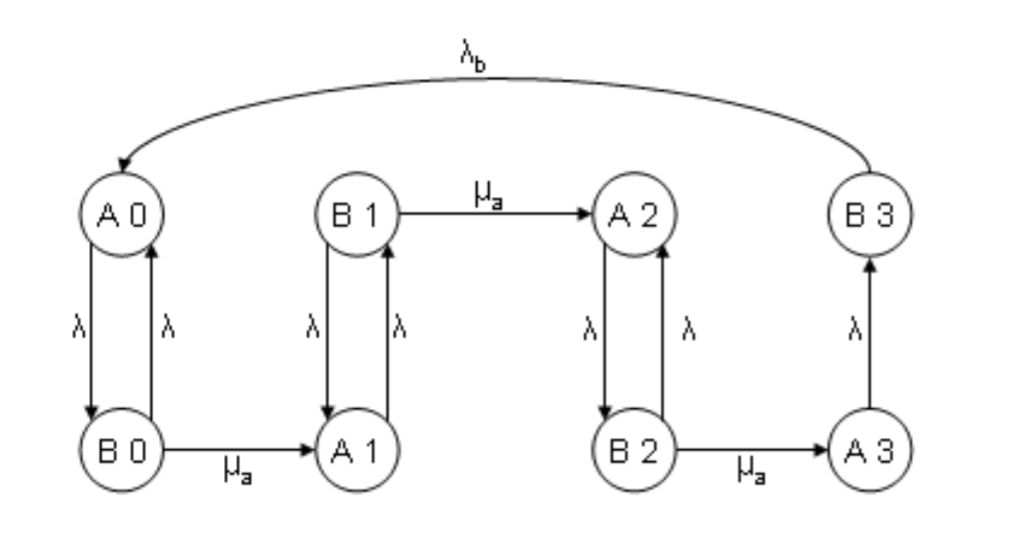
\includegraphics[width=0.7\textwidth]{img/ejemplo.png}
  \caption{CMTD asociada al ejemplo}
  \label{fig:ejemplo}
\end{figure}
\end{document}}